\documentclass[]{article}
\usepackage[spanish.mexico]{babel}
\usepackage[T1]{fontenc}
\usepackage[utf8]{inputenc}
\usepackage{lmodern}
\usepackage[a4paper]{geometry}

\usepackage{hyperref}
%Enclaces
\hypersetup{
	colorlinks=true,
	linkcolor=blue,
	filecolor=magenta,      
	urlcolor=cyan,
}

\urlstyle{same}

\usepackage{graphicx}
\usepackage{cite}

%DIAGRAMA DE GANT 
\usepackage{pgfgantt}
%\usepackage{graphicx}
\usepackage{xcolor}
%\usepackage[spanish.mexico]{babel}
%\usepackage[utf8]{inputenc}
%\usetikzlibrary{positioning}

\ganttset{group/.append style={orange},
	milestone/.append style={red},
	progress label node anchor/.append style={text=red}}

%%MULTICOL


\usepackage{etoolbox,refcount}
\usepackage{multicol}

\newcounter{countitems}
\newcounter{nextitemizecount}
\newcommand{\setupcountitems}{%
	\stepcounter{nextitemizecount}%
	\setcounter{countitems}{0}%
	\preto\item{\stepcounter{countitems}}%
}
\makeatletter
\newcommand{\computecountitems}{%
	\edef\@currentlabel{\number\c@countitems}%
	\label{countitems@\number\numexpr\value{nextitemizecount}-1\relax}%
}
\newcommand{\nextitemizecount}{%
	\getrefnumber{countitems@\number\c@nextitemizecount}%
}
\newcommand{\previtemizecount}{%
	\getrefnumber{countitems@\number\numexpr\value{nextitemizecount}-1\relax}%
}
\makeatother    
\newenvironment{AutoMultiColItemize}{%
	\ifnumcomp{\nextitemizecount}{>}{3}{\begin{multicols}{2}}{}%
		\setupcountitems\begin{itemize}}%
		{\end{itemize}%
		\unskip\computecountitems\ifnumcomp{\previtemizecount}{>}{3}{\end{multicols}}{}}


\title{Electrónica Básica con Texas Instruments Tiva Launchpad}
\author{Pablo Vivar Colina}
%\date{October 2015}




\begin{document}



\maketitle

%\begin{figure}[h!]
%	\centering
%	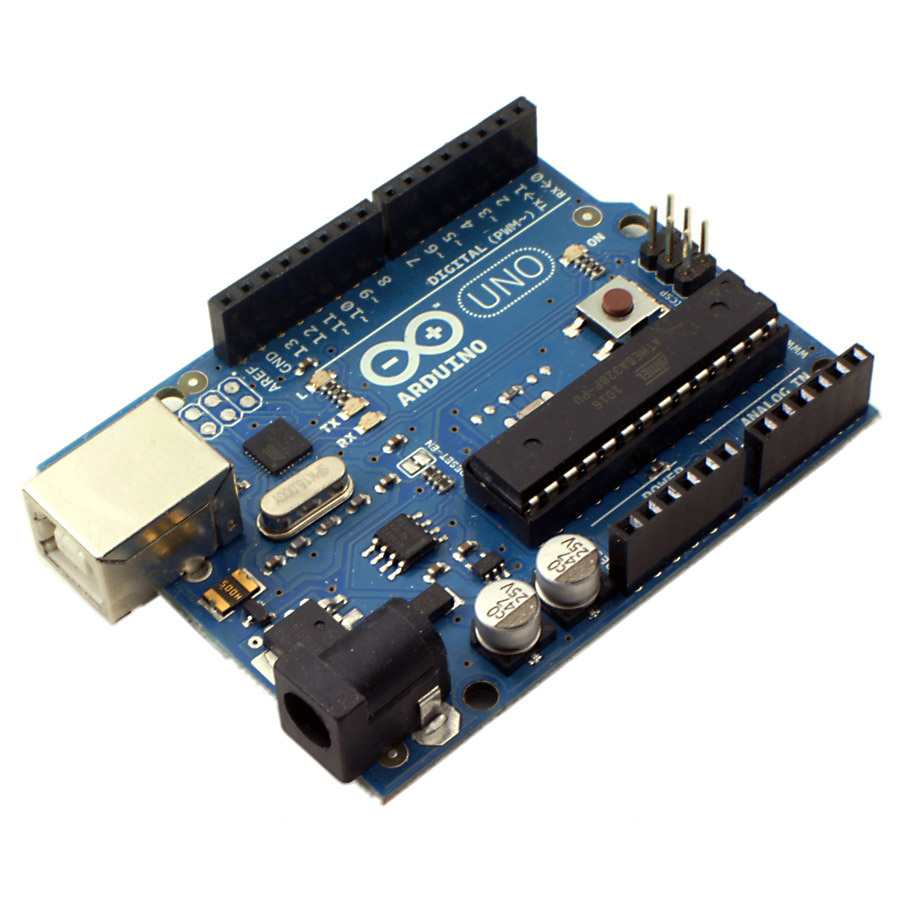
\includegraphics[width=0.15\textwidth]{Arduino_Uno_Angle}
%\end{figure}

\begin{figure}[h!]
	\centering
	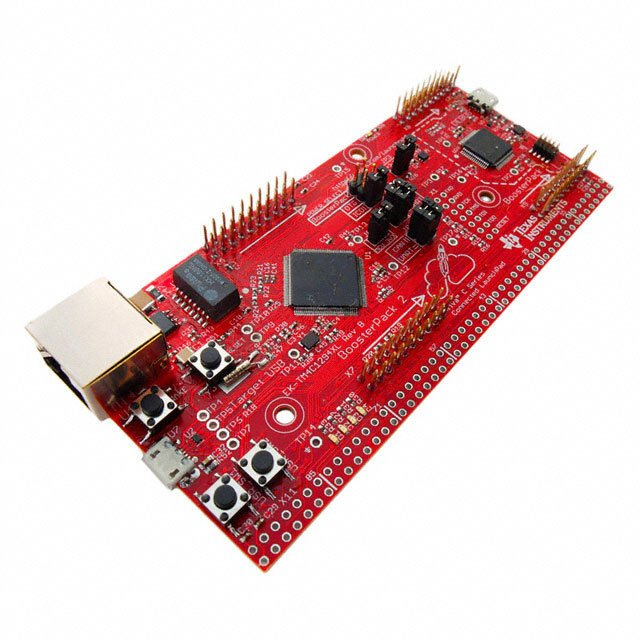
\includegraphics[width=0.15\textwidth]{MFG_EK-TM4C1294XL}
\end{figure}

%NUEVA TABLA

\begin{table}[h!]
	\centering
	\begin{tabular}{||c|l||}
		
		%Filas
		%objetivos
		%Audiencia
		%equipo
		%costo
		%tiempo
		%venue  (involucrados) biblioteca benjamín franklin
		%outcome (logros) desarrollar un robot ensamblado con piezas 3D y hacerlo funcionar arduino
		
		%3D piezas como regalo
		
		
		%\begin{enumerate}
		%	\item Usar tecnologías de microcontroladores como la que provee el desarrollo de tarjetas open source Arduino para realizar prototipos electromecánicos que puedan resolver tareas en específico.
		%	\item Describir conceptos de electrónica, mecanismos y de programación en el nivel suficiente para la elaboración de prototipos.
		%	\item Describir nuevas tecnologías como la impresión en 3D para realizar componentes físicos en la elaboración de un sistema electromecánico.
		%\end{enumerate}
		
		
		
		\hline
		\textbf{Section} & \multicolumn{1}{|c|}{\textbf{Description}}       \\[0.5ex]\hline\hline
				
		\textbf{Objectives} & The attendant will get experience with:    \\[0.5ex] 
		& $\bullet$ Free software programs and Technologies as 3D printers \\[0.5ex]
		& $\bullet$ Programming environments and microcontrollers applications\\[0.5ex]
		
			& $\bullet$ Building a functional electromechanical prototype like a zumo bot\\[0.5ex]
		\hline
		
		\textbf{Attendants} &  Teenagers between 14 and 18 years   \\[0.5ex]
		& People who is interested in electronics and maker topics   \\[0.5ex]
		& The workshop group is for 15 attendants    \\[0.5ex] \hline
		
		\textbf{Equipment} & Laptop computers, Launch Pad board and electronic materials  \\[0.5ex] \hline
		
		\textbf{Costs} & 15 kits (complete group)  1833.15[USD]  \\[0.5ex] 
		& 35814.8[MXN]  \\[0.5ex] \hline
		
		\textbf{Time} & 40 hours\\[0.5ex]
		             & 10 sessions (2 hours per week)   \\[0.5ex]
		 \hline
		
		\textbf{Venue} & Biblioteca Benjamín Franklin,\\[0.5ex]  
	                   & IDEA 1.61, DITAC, LIDSOL  	\\[0.5ex] \hline
		
		\textbf{Outcome} &    The attendant will:\\[0.5ex]
		& $\bullet$ Ensamble a robot with 3D printed parts (keep the parts to make the robot at home). \\[0.5ex]
		& $\bullet$ Code to make the robot work. \\[0.5ex] 
		& $\bullet$ Test the robot . \\[0.5ex]
	    & The library will:\\[0.5ex]
	    &  $\bullet$ Get involved with high school attendants \\[0.5ex]
	    &  $\bullet$ Get Development boards to porgramming workshops \\[0.5ex]
	    &  $\bullet$ Get electronic material for this workshop and further more engenieering workshops. \\[0.5ex]
		\hline
		
	\end{tabular}
	\caption{Summary}
	
\end{table}

\section{Introducción}

En el curso se encuentran mostradas dos propuestas de tarjeta de desarrollo, pero la versatilidad de la tecnología del presente nos brinda la oportunidad de trabajar con ambas tarjetas de desarrollo con facilidad con prácticamente el mismo entorno de desarrollo y usando el mismo lenguaje de programación.\\

A lo largo del documento se muestra orientado hacia la tarjeta de desarrollo Tiva Launchpad ya que la recomiendo como mejor alternativa que la tarjeta Arduino porque el hardware que se le incluye es mucho más poderoso y además que se presta para muchas más aplicaciones.\\

La tarjeta Tiva Launchpad además se puede utilizar para futuros cursos que se enseñe a programar con el lenguaje de C a nivel de hardware, como es utilizado actualmente en la industria.\\

La biblioteca se verá beneficiada con todo el material de componentes de electrónica ya que son compatibles con todas las tarjetas de desarrollo en el mercado, y además el participante podrá quedarse con las piezas en 3D elaboradas en el taller y podrá armar el mismo prototipo que armó en el taller en casa ya que la mayoría de los componentes electrónicos son fáciles de adquirir.\\

Si el participante quiere replicar lo visto en el curso con una tarjeta arduino es totalmente posible ya que podrá identificar los componentes funcionales y el software utilizado es prácticamente idéntico.\\

\subsection{Energia (Texas Instruments)}

%What is Energia and how did it get started\cite{TX}\\

Energia is an open-source electronics prototyping platform started by Robert Wessels in January of 2012 with the goal to bring the Wiring and Arduino framework to the Texas Instruments MSP430 based LaunchPad. The Energia IDE is cross platform and supported on Mac OS, Windows, and Linux. Energia uses the mspgcc compiler by Peter Bigot and is based on the Wiring and Arduino framework. Energia includes an integrated development environment (IDE) that has it’s foundation in the Processing IDE (Processing->Wiring->Arduino->Energia). Energia is also a portable framework/abstraction layer that can be used in other popular IDEs. Utilize a web browser based environment with Texas Instruments CCS Cloud at dev.ti.com or TI’s powerfull CCS Desktop IDE.\cite{TX}\\

The foundation of Energia and Arduino is the Wiring framework that was developed by Hernando Barragan. The framework is thoughtfully created with designers and artists in mind to encourage a community where both beginners and experts from around the world share ideas, knowledge and their collective experience. The Energia team adopts the philosophy of learning by doing and strives to make it easy to work directly with the hardware. Professional engineers, entrepreneurs, makers, and students can all benefit from the ease of use Energia brings to the microcontroller.\cite{TX}\\

Energia started out to bring the Wiring and Arduino framework to the Texas Instruments MSP430 LaunchPad. Texas Instruments offers a MSP430, MSP432x, TM4C, C2000, CC32xx and CC13xx LaunchPad. The LaunchPad is a low-cost microcontroller board that is made by Texas Instruments. The latest release of Energia supports the majority of the LaunchPad product offerings.

Together with Energia, LaunchPad can be used to develop interactive objects, taking inputs from a variety of switches or sensors, and controlling a variety of lights, motors, and other physical outputs. LaunchPad projects can be stand-alone (only run on the Target Board, i.e. your LaunchPad), or they can communicate with software running on your computer (Host PC). You can also add wireless modules to enable communication over various types of RF including Wi-Fi, NFC, Bluetooth, Zigbee, cellular, and more.\cite{TX}\\

%More information about LaunchPad can be found on the TI site: www.ti.com/launchpad
%Getting Started

%To get started with Energia for your operating system (Energia works on Mac OS X, Linux and Windows), follow the instructions in the getting started guide. Start learning by doing using the handy tutorials and example code provided in the tutorial section of the getting started guide. You can find important board setup instructions and pin maps on the right hand navigation links of the website.\cite{TX}\\

%The Energia APIs are documented in the reference section. Find out how the core functions and library functions operate to be a more effective programmer.\cite{TX}\\

\subsection{Arduino}

Arduino es una plataforma de hardware libre, basada en una placa con un microcontrolador y un entorno de desarrollo, diseñada para facilitar el uso de la electrónica en proyectos multidisciplinares.\cite{Ard}\\

%El hardware consiste en una placa con un microcontrolador Atmel AVR y puertos de entrada/salida.4 Los microcontroladores más usados son el Atmega168, Atmega328, Atmega1280, y Atmega8 por su sencillez y bajo coste que permiten el desarrollo de múltiples diseños. Por otro lado el software consiste en un entorno de desarrollo que implementa el lenguaje de programación Processing/Wiring y el cargador de arranque que es ejecutado en la placa.4 Se programa en el ordenador para que la placa controle los componentes electrónicos.\cite{Ard}\\

%Desde octubre de 2012, Arduino se utiliza también con microcontroladoras CortexM3 de ARM de 32 bits,5 que coexistirán con las más limitadas, pero también económicas AVR de 8 bits. ARM y AVR no son plataformas compatibles a nivel binario, pero se pueden programar con el mismo IDE de Arduino y hacerse programas que compilen sin cambios en las dos plataformas. Eso sí, las microcontroladoras CortexM3 usan 3,3V, a diferencia de la mayoría de las placas con AVR, que generalmente usan 5V. Sin embargo, ya anteriormente se lanzaron placas Arduino con Atmel AVR a 3,3V como la Arduino Fio y existen compatibles de Arduino Nano y Pro como Meduino en que se puede conmutar el voltaje.\cite{Ard}\\

Arduino puede tomar información del entorno a través de sus entradas analógicas y digitales, puede controlar luces, motores y otros actuadores. El microcontrolador en la placa Arduino se programa mediante el lenguaje de programación Arduino (basado en Wiring) y el entorno de desarrollo Arduino (basado en Processing). Los proyectos hechos con Arduino pueden ejecutarse sin necesidad de conectar a un ordenador.\cite{Ard}\\

También cuenta con su propio software que se puede descargar de su página oficial que ya incluye los drivers de todas las tarjetas disponibles lo que hace más fácil la carga de códigos desde el computador.\cite{Ard}\\

%Arduino se puede utilizar para desarrollar objetos interactivos autónomos o puede ser conectado a software tal como Adobe Flash, Processing, Max/MSP, Pure Data. Una tendencia tecnológica es utilizar Arduino como tarjeta de adquisición de datos desarrollando interfaces en software como JAVA, Visual Basic y LabVIEW 6 . Las placas se pueden montar a mano o adquirirse. El entorno de desarrollo integrado libre se puede descargar gratuitamente.\cite{Ard}\\

%termina arduino

\subsection{Software Libre}

El software libre suele estar disponible gratuitamente, o al precio de coste de la distribución a través de otros medios; sin embargo no es obligatorio que sea así, por lo tanto no hay que asociar «software libre» a «software gratuito» (denominado usualmente freeware), ya que, conservando su carácter de libre, puede ser distribuido comercialmente. Análogamente, el software gratis o gratuito incluye en ocasiones el código fuente; no obstante, este tipo de software no es «libre» en el mismo sentido que el software libre, a menos que se garanticen los derechos de modificación y redistribución de dichas versiones modificadas del programa.\cite{SL}\\

Tampoco debe confundirse software libre con «software de dominio público». Éste último es aquel que no requiere de licencia, pues sus derechos de explotación son para toda la humanidad, porque pertenece a todos por igual. Cualquiera puede hacer uso de él, consignando su autoría original. Este software sería aquel cuyo autor lo dona a la humanidad o cuyos derechos de autor han expirado. Si un autor condiciona su uso bajo una licencia, por muy débil que sea, ya no es del dominio público.\cite{SL}\\

\section{Público}

El curso está diseñado para asistentes que estén cursando la secundaria o la preparatoria, es decir con edades recomendadas de entre 14 y 18 años, con aptitudes para temas de electrónica, progamación y entusiasmo en realizar prototipos físicos.\\

% First meeting\\
%	 & Pablo \\ \hline

%Éste tema tiene como objetivo introducir los conceptos básicos como software libre, tarjetas de desarrollo, las capacidades de la tarjeta de desarrollo arduino. Además de explicar brevemente las funcionalidades que incluye

% Además de explicar brevemente las funcionalidades que incluye\\

%	En éste tema se describirán los componentes que se utilizarán a lo largo del curso, su funcionamiento, correcta polarización y notas correspondientes.\\

%	Se verificará también la correcta instalación y funcionamiento del software necesario en el curso.\\

%En ésta sesión se dará una breve introducción sobre los diagramas de bloques de programación, soluciones de algunos problemas a través de algoritmos. Se implementará el programa visto en código que funcionará en la tarjeta Arduino.\\

\section{El alumno tendrá habilidades para:}

%INFINITIVO EL alumno podrá o tendra habilidades para...
\begin{enumerate}
    \item Usar tecnologías de microcontroladores como la que provee el desarrollo de tarjetas open source Arduino para realizar prototipos electromecánicos que puedan resolver tareas en específico.
    \item Describir conceptos de electrónica, mecanismos y de programación en el nivel suficiente para la elaboración de prototipos.
    \item Describir nuevas tecnologías como la impresión en 3D para realizar componentes físicos en la elaboración de un sistema electromecánico.
\end{enumerate}

\section{Hardware necesario}


\subsection{Provisto en el Taller}

\begin{enumerate}
	\item Impresora 3D.
	\item PLA para piezas a elaborar.
	\item Computadora Laptop.
  %\item Componentes electrónicos.
\end{enumerate}

%Cuestionario de seleccion
%eventbrite lugares
%SOLICITAR A LOS ASISTENTES COMPUTADORA

%Promocion plataformas de la bibleteca, plataforma de idea y de lidsol

\subsubsection{Componentes electrónicos}


\begin{table}[h!]
	\centering
	\begin{tabular}{||c|c|c||}
		\hline
		\textbf{Parte} & \textbf{Cantidad}     & \textbf{Costo USD}      \\ \hline\hline
		%\href{https://www.digikey.com.mx/product-detail/es/arduino/A000066/1050-1024-ND/2784006}{Arduino UNO} & 1 & 23.38 \\ \hline 
		
		\href{https://www.digikey.com.mx/product-detail/es/texas-instruments/EK-TM4C1294XL/296-37267-ND/4725808}{ EK-TM4C1294XL} & 1 & 20.76 \\ \hline 
		\href{https://www.digikey.com.mx/product-detail/es/pimoroni-ltd/PIM244/PIM244-ND/8126061}{LED y resistores diversos}  & 1 &  6.65   \\ \hline
		\href{https://www.digikey.com.mx/product-detail/es/global-specialties/GS-830/BKGS-830-ND/5231309}{Breadboard} & 1 &  8.25   \\ \hline
		\href{https://www.digikey.com.mx/product-detail/es/bud-industries/BC-32625/377-2093-ND/4156446}{Cables jumper} & 1 & 5.3    \\ \hline
		\href{https://www.digikey.com.mx/product-detail/es/c-k/PTS-647-SM50-SMTR2-LFS/PTS647SM50SMTR2LFSDKR-ND/9649876}{Push button} & 7 & 0.14    \\ \hline
		\href{https://www.digikey.com.mx/product-detail/es/bourns-inc/3310R-125-103L/3310R-125-103L-ND/2537840}{Potenciómetro} & 1 &  2.74  \\ \hline
		\href{https://www.digikey.com.mx/product-detail/es/adafruit-industries-llc/169/1528-1076-ND/5154651}{Servomotor} & 1 &  5.95   \\ \hline
		\href{https://www.digikey.com.mx/product-detail/es/vishay-semiconductor-opto-division/TCST2202/TCST2202-ND/1681171}{Sensor óptico} & 1 & 1.86    \\ \hline
		\href{https://www.digikey.com.mx/product-detail/es/sparkfun-electronics/SEN-13959/1568-1421-ND/6193598}{Sensor Ultrasónico} & 1 &  3.95   \\ \hline
		\href{https://www.digikey.com.mx/product-detail/es/digilent-inc/410-069/1286-1139-ND/4090146}{Puente H} & 1 & 9.99     \\ \hline
		\href{https://www.digikey.com.mx/product-detail/es/adafruit-industries-llc/3777/1528-2589-ND/8687221}{Motor Reductor} & 2 & 2.95    \\ \hline
		\href{https://tinyurl.com/sllgmt5}{Módulo bluetooth}	 & 1 & 12.92    \\ \hline
		\href{https://www.digikey.com.mx/product-detail/es/mpd-memory-protection-devices/BH4AAW/BH4AA-W-ND/32051}{Portapilas AA} & 1 & 3.72    \\ \hline
		   \href{https://www.digikey.com.mx/product-detail/es/energizer-battery-company/CHPROWB4/N734-ND/7403296}{Baterías Recargables y cargador} & 1 &  19.92   \\ \hline
		  \textbf{Total 1 Asistente} & & 108.89 USD\\ \hline
		   \textbf{Total 15 Asistentes} & & 1633.35 USD\\ \hline
		   \textbf{Total 15 Asistentes} & &   30,705.76  MXN\\ \hline
	\end{tabular}
	\caption{Costos Componentes Electrónicos por asistente}
	\label{costos}
\end{table}

En el cuadro \ref{costos} se enumeran los componentes utilizados por asistente además de las cantidades a ocupar y precios, el total mostrado corresponde al material. En el entendido que el curso está pensado para 15 asistentes el nuevo total es de 1833.15 USD equivalentes a 35814.8 MXN. Es importante notar que en la suma sólo se contempla el Arduino UNO como tarjeta de desarrollo, pero no se agrega al costo la tarjeta Tiva Launchpad (EK-TM4C1294XL), esto pensando que se tome en cuenta el precio de la tarjeta de desarrollo a el mayor precio. \\

%COSTOS
%mostrar precios y multiplicar por 15 asistentes 

\section{Software necesario}

\begin{itemize}
	
	\item \href{https://energia.nu/download/}{Energia IDE}
    \item \href{https://www.arduino.cc/en/Main/Software}{Arduino IDE}
    \item \href{http://www.openscad.org}{OpenSCAD (opcional)}
\end{itemize}

\section{Temario}

El curso comprende 10 sesiones de 2 horas cada una, en las que se verán los temas que se presentan a continuación. En los cuadros \ref{cuadroCurso0} y \ref{cuadroCurso1} se describirá la distribución de los temas mostrados en el orden de las sesiones.\\

\subsection{Introducción}\label{subcap:Intro}

El curso tiene como objetivo que el alumno conozca los conceptos básicos como software libre, tarjetas de desarrollo, open source y Arduino, así como, explicar brevemente las funcionalidades que incluye.

\subsection{Electrónica básica}\label{subcap:Ebas}

Se describirán los componentes que se utilizarán a lo largo del curso, su funcionamiento, correcta polarización y notas correspondientes.\\

Se verificará también la correcta instalación y funcionamiento del software necesario en el curso.\\

\subsection{Fundamentos de programación}\label{subcap:FunPro}

Se dará una breve introducción sobre los diagramas de bloques de programación, soluciones de algunos problemas a través de algoritmos. Se implementará el programa visto en código que funcionará en la tarjeta Arduino.\\

\subsection{Salidas digitales}\label{subcap:SalDigital}

Se dará una breve explicación sobre el concepto de entradas y salidas digitales, además se utilizará el entorno de desarrollo de Arduino, para realizar las primeras pruebas con los pines.\\

En conjunto se implementará el monitor serial de la tarjeta entre otras utilidades.\\

\subsection{Entradas digitales}\label{subcap:EntDigital}

Se utilizará el entorno de desarrollo de Arduino para realizar las primeras lecturas a través de los pines de entrada de la tarjeta, se retomará la utilización del monitor serial y se complementará con los conocimientos anteriores.\\

\subsection{Entradas analógicas}\label{subcap:EntAnalog}

Se retomarán los conceptos anteriormente vistos y se realizarán diferentes lecturas analógicas con diferentes tipos de sensores.\\

Se realizará el código correspondiente para la correcta caracterización de los sensores anteriormente probados.\\

\subsection{Salidas analógicas}\label{subcap:SalAnalog}

Se dará una breve introducción sobre el concepto de PWM y sus aplicaciones con componentes como un servomotor o un LED. Además de que se realizarán códigos que integren conceptos anteriormente vistos como el monitor serial y entradas analógicas para su aplicación en conjunto.\\

\subsection{Diseño 3D OpenSCAD}\label{subcap:OpenSCAD}

Se dará una breve introducción al modelado parametrizable con OpenSCAD, también se explicará la interfaz de usuario del programa y los diseños que se encuentran disponibles en línea.\\ 

\subsection{Elaboración de proyecto}\label{subcap:Proyecto}

Se reunirán los conocimientos obtenidos a lo largo del curso para realizar un prototipo electromecánico funcional.


\section{Colaboradores}

\subsection{IDEA 1.61}

Empresa cofundada en 2017, dedicada al desarrollo tecnológico a través de la implementación y uso de nuevas tecnologías como las impresoras 3D y máquinas de corte láser.\\

Impresión 3D: Ve tu diseño convertirse en realidad al imprimirlo en 3D. Nuestras máquinas ocupan tecnología de Fused Deposition Modeling (FDM) para obtener la mejor calidad al mejor precio. Todas las impresiones son totalmente personalizadas.\\

Desarrollo de Proyectos: Tu que quieres quieres crear algo, no te preocupes por los detalles. Nosotros podemos asistirte con tus proyectos escolares al igual que profesionales. Contamos con un equipo de ingenieros especializados en diferentes ramas para asegurar la más alta calidad en tu proyecto.\\

\subsection{DITAC}

Empresa fundada en 2016, dedicada a la elaboración de piezas modulares para prototipos físicos experimentales. Principalemte orientadas hacia la creación de prototipos físicos experimentales.\\

\subsection{LIDSOL}

LIDSOL es un laboratorio de la Facultad de Ingeniería de la UNAM, establecido en 2001, formado por voluntarios, alumnos, ex-alumnos y académicos interesados en el desarrollo de tecnologías libres y las discusiones sobre su impacto en la sociedad.\\

Buscamos promover e impulsar la investigación y desarrollo de tecnologías libres realizando proyectos afines en distintas áreas buscando el progreso y mejoramiento de la sociedad.\\


\section{Programa}

En los cuadros \ref{cuadroCurso0} y \ref{cuadroCurso1} se pueden apreciar los días en que serán llevadas acabo las sesiones además de los objetivos en específico de cada una y puede apreciarse los temas que serán cubiertos.\\



\begin{table}[h!]
	\centering
	\begin{tabular}{|c|l|c|}
		\hline
		\textbf{Date} & \multicolumn{1}{c}{\textbf{Task}}  & \textbf{Presenter}      \\ \hline
		23 October & First Session, this activity pretend to:   & Pablo     \\ 
		16:30 to 18:30 & $\bullet$ Introduce the objective and session program of the course &     \\
		& $\bullet$ Explain Launchpad board and free software concepts &     \\ 
		& $\bullet$ Make a brief overview of electronic hardware & \\
		& sections(\ref{subcap:Intro},\ref{subcap:Ebas})& \\ \hline
		
		30 October & Second Session, this activity pretend to:  & Pablo \\
		16:30 to 18:30     & 	$\bullet$ Explain Pins on Arduino/Launchpad board. &     \\
		& $\bullet$ Make introduction to programming basics with Arduino/Energia IDE &  \\ 
		& $\bullet$ The student can make the first $"hello$ $world"$ sketch & \\ 
		& sections(\ref{subcap:Ebas},\ref{subcap:FunPro})&  \\ \hline
		
		6 November & Third Session, this activity pretend to: & Pablo \\
		16:30 to 18:30	 & 	$\bullet$ Explain Digital input and output system &     \\
		& $\bullet$ Wire push button circuit as digital input &     \\  
		& $\bullet$ Wire LED as digital output &\\ 
		& $\bullet$ Make sketch that makes electronic hardware work & \\ 
		& sections(\ref{subcap:EntDigital},\ref{subcap:SalDigital})& \\ \hline
		
		13 November & Fourth Session, this activity pretend to:  & Pablo \\ 
		16:30 to 18:30 & $\bullet$ Explain Serial monitor concept &     \\
		& $\bullet$ Integrate Serial monitor to previous sketch &     \\ 
		& sections(\ref{subcap:SalDigital}) & \\ \hline
		
		20 November & Finfth Session, this activity pretend to: & Pablo \\ 
		16:30 to 18:30 & $\bullet$ Wire potentiometer circuit &     \\
		& $\bullet$ Wire LED as analog output  &     \\ 
		& $\bullet$ Make sketch that makes electronic hardware work & \\
		& sections(\ref{subcap:EntAnalog},\ref{subcap:SalAnalog}) & \\ \hline
		
	\end{tabular}
	\caption{First Half Activities Calendar}
	\label{cuadroCurso0}
\end{table}

\begin{table}[h!]
	\centering
	\begin{tabular}{|c|l|c|}
		\hline
		\textbf{Date} & \multicolumn{1}{c}{\textbf{Task}}     & \textbf{Presenter}      \\ \hline
		27 November & Sixth Session, this activity pretend to: & Pablo     \\ 
		16:30 to 18:30 & $\bullet$ Wire servo as analog output &     \\
		& $\bullet$ Make sketch that makes electronic hardware work &     \\ 
		& sections(\ref{subcap:SalAnalog})& \\ \hline
		4 December & Seventh Session, this activity pretend to: & Pablo \\
		16:30 to 18:30     & $\bullet$ Explain how Ultra Sonic Sensor Work &     \\
		& $\bullet$  Wire Ultra Sonic Sensor to Arduino/Launchpad board &     \\ 
		& $\bullet$  Make a sketch that makes UltraSonic sensor works & \\
		&sections(\ref{subcap:SalDigital},\ref{subcap:SalDigital})& \\ \hline
		11 December & Eighth Session, this activity pretend to: & Pablo \\
		16:30 to 18:30	 & $\bullet$ Make a brief explanation of 3D printing process & \\
		 & 	$\bullet$ Introduce to 3D design in OpenSCAD &     \\
		  & $\bullet$ Explain Thingiverse 3D parts collection &     \\
		& $\bullet$ Prepare 3D printed parts for further use &     \\  
		& sections(\ref{subcap:OpenSCAD})&\\ \hline
		
		18 December & Ninth Session, this activity pretend to: & Pablo \\ 
		16:30 to 18:30 & $\bullet$ Explain Hdirver function &     \\
		& $\bullet$ Wire Hdiver to Launchpad board &     \\ 
		& $\bullet$ Make a sketch that makes hardware work & \\ 
		& sections(\ref{subcap:SalDigital})& \\ \hline
		
	    25 December& Tenth Session, this activity pretend to: & Pablo \\ 
		16:30 to 18:30 & $\bullet$ Integrate electronic hardware with 3D printed parts &     \\
		& $\bullet$ Test and run the prototype&     \\ 
		& sections(\ref{subcap:Proyecto}) & \\ \hline
		
	\end{tabular}
	\caption{Second Half Activities Calendar}
	\label{cuadroCurso1}
\end{table}



\subsection{Diagrama de Gant}

\begin{figure}[h!]
	
	\begin{ganttchart}[%Specs
		y unit title=0.5cm,
		y unit chart=0.7cm,
		vgrid,hgrid,
		title height=1,
		%     title/.style={fill=none},
		title label font=\bfseries\footnotesize,
		bar/.style={fill=blue},
		bar height=0.7,
		%   progress label text={},
		group right shift=0,
		group top shift=0.7,
		group height=.3,
		group peaks width={0.2},
		inline]{1}{25}
		%labels
		%\gantttitle{Tema 1}{31}\\  % title 1
		\gantttitle[]{Octubre/Noviembre}{25}\\                 % title 2
		
		\gantttitle{1st Day 23 Oct}{5}                      % title 3
		\gantttitle{2nd Day 30 Oct}{5}
		\gantttitle{3rd Day 6 Nov}{5}
		\gantttitle{4th Day 13 Nov}{5}
		\gantttitle{5th Day 20 Nov}{5}
		%\gantttitle{Q3}{6}
		%\gantttitle{Q4}{6}
		\\
		% Setting group if any
		\ganttgroup[inline=false]{I}{1}{5}\\ 
		\ganttbar[progress=1,inline=false]{Prgs}{1}{5}\\
		\ganttmilestone[inline=false]{S1}{3} \\
		
		
		\ganttgroup[inline=false]{II}{6}{10}\\ 
		\ganttbar[progress=0,inline=false]{Prgs}{6}{10}\\
		\ganttmilestone[inline=false]{S2}{8} \\
				
				
	 \ganttgroup[inline=false]{III}{11}{15}\\ 
	 \ganttbar[progress=0,inline=false]{Prgs}{11}{15}\\
	 \ganttmilestone[inline=false]{S3}{13} \\
				
				
	 \ganttgroup[inline=false]{IV}{16}{20}\\ 
	 \ganttbar[progress=0,inline=false]{Prgs}{16}{20}\\
	 \ganttmilestone[inline=false]{S4}{18} \\
				
				
	\ganttgroup[inline=false]{V}{21}{25}\\ 
	\ganttbar[progress=0,inline=false]{Prgs}{21}{25}\\
	\ganttmilestone[inline=false]{S5}{23} \\
				
				
	\end{ganttchart}
	\caption{Sesiones}
	\label{fig:diagGant0}
\end{figure}


\begin{figure}[h!]
	
	\begin{ganttchart}[%Specs
		y unit title=0.5cm,
		y unit chart=0.7cm,
		vgrid,hgrid,
		title height=1,
		%     title/.style={fill=none},
		title label font=\bfseries\footnotesize,
		bar/.style={fill=blue},
		bar height=0.7,
		%   progress label text={},
		group right shift=0,
		group top shift=0.7,
		group height=.3,
		group peaks width={0.2},
		inline]{1}{25}
		%labels
		%\gantttitle{Tema 1}{31}\\  % title 1
		\gantttitle[]{Noviembre/Diciembre}{25}\\                 % title 2
		
		\gantttitle{6th Day 27 Nov}{5}                      % title 3
		\gantttitle{7th Day 4 Dic}{5}
		\gantttitle{8th Day 11 Dic}{5}
		\gantttitle{9th Day 18 Dic}{5}
		\gantttitle{10th Day 25 Dic}{5}
		%\gantttitle{Q3}{6}
		%\gantttitle{Q4}{6}
		\\
		% Setting group if any
		\ganttgroup[inline=false]{I}{1}{5}\\ 
		\ganttbar[progress=1,inline=false]{Prgs}{1}{5}\\
		\ganttmilestone[inline=false]{S6}{3} \\
		
		
		\ganttgroup[inline=false]{II}{6}{10}\\ 
		\ganttbar[progress=0,inline=false]{Prgs}{6}{10}\\
		\ganttmilestone[inline=false]{S7}{8} \\
		
		
		\ganttgroup[inline=false]{III}{11}{15}\\ 
		\ganttbar[progress=0,inline=false]{Prgs}{11}{15}\\
		\ganttmilestone[inline=false]{S8}{13} \\
		
		
		\ganttgroup[inline=false]{IV}{16}{20}\\ 
		\ganttbar[progress=0,inline=false]{Prgs}{16}{20}\\
		\ganttmilestone[inline=false]{S9}{18} \\
		
		
		\ganttgroup[inline=false]{V}{21}{25}\\ 
		\ganttbar[progress=0,inline=false]{Prgs}{21}{25}\\
		\ganttmilestone[inline=false]{S10}{23} \\
		
		
	\end{ganttchart}
	\caption{Sesiones}
	\label{fig:diagGant1}
\end{figure}


En las figuras \ref{fig:diagGant0} y \ref{fig:diagGant1}  Se muestra el desarrollo cronológico de las sesiones en el transcurso de un mes, los días hábiles se encuentran señalizados en naranja. Las sesiones tendrían lugar los días miércoles de cada semana, el cual se encuentra marcado con un diamante rojo.\\


\bibliographystyle{plain}
\bibliography{referencias.bib}


\end{document}
